\documentclass[10pt,a4paper]{article}
\usepackage[margin=0.8in]{geometry}
\usepackage{multicol}
\usepackage{amsmath}
\usepackage{tikz}
\usepackage{enumitem}
\usepackage{titlesec}
\usepackage{fontspec}
\usepackage{lipsum}

% Compact formatting
\setlength{\columnsep}{0.7cm}
\setlength{\parindent}{0pt}
\setlength{\parskip}{0.1cm}
\titlespacing{\section}{0pt}{0.3cm}{0.1cm}
\titlespacing{\subsection}{0pt}{0.2cm}{0.05cm}

% Custom section style
\titleformat{\section}{\large\bfseries}{}{0em}{}
\titleformat{\subsection}{\normalsize\bfseries}{}{0em}{}

\begin{document}

\begin{center}
{\LARGE \textbf{Economics: Basic Concepts}}\\[0.2cm]
\textit{Topic 1: Foundations of Economic Thought}
\end{center}
\vspace{-0.3cm}

\begin{multicols}{2}
\footnotesize

% --- DEFINITION ---
\section*{Definition}
\textbf{Economics} is the social science studying how individuals, businesses, and societies allocate \textbf{scarce resources} to satisfy \textbf{unlimited wants}. It analyzes production, distribution, and consumption of goods/services.

\textbf{Scope:} Spans from individual choices (micro) to national policies (macro), covering markets, growth, unemployment, inflation, and global trade.

% --- HOW TO REMIND ---
\subsection*{Memory Triggers}
\begin{itemize}[leftmargin=*,nosep]
    \item \textbf{``Scarce Resources + Unlimited Wants = Economics''} -- The fundamental equation.
    \item \textbf{``No Free Lunch''} (TANSTAAFL) -- Every choice involves a cost.
    \item \textbf{Three Questions:} \textit{What, How, For Whom} to produce? -- Core of economic systems.
\end{itemize}

% --- MATHEMATICAL TERM ---
\subsection*{Mathematical Representation}
\textbf{Opportunity Cost (Explicit Formula):}
\[
OC_x = \frac{\text{Loss in Good Y}}{\text{Gain in Good X}}
\]
\textbf{Production Possibility Frontier (PPF):} Shows maximum output combos. Slope = Marginal Rate of Transformation (MRT).
\[
MRT = -\frac{dy}{dx} = \frac{MC_x}{MC_y}
\]
Moving along the PPF, increasing production of X requires sacrificing Y -- this is the \textbf{tradeoff}.

% --- GRAPH STUDY ---
\subsection*{Graph Study: Production Possibility Frontier}
\begin{center}
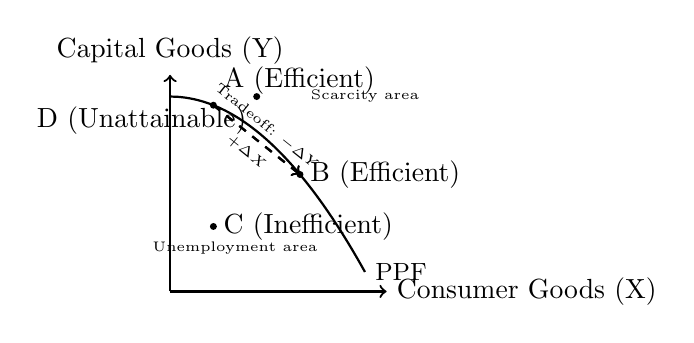
\begin{tikzpicture}[scale=0.55, thick]
    % Axes
    \draw[->] (0,0) -- (5,0) node[right] {Consumer Goods (X)};
    \draw[->] (0,0) -- (0,5) node[above] {Capital Goods (Y)};
    % PPF Curve
    \draw[domain=0:4.5, smooth] plot (\x, {4.5 - 0.2*\x*\x}) node[right] {\small PPF};
    % Points
    \filldraw (1,4.3) circle (1.5pt) node[above right] {A (Efficient)};
    \filldraw (3,2.7) circle (1.5pt) node[right] {B (Efficient)};
    \filldraw (2,4.5) circle (1.5pt) node[below left] {D (Unattainable)};
    \filldraw (1,1.5) circle (1.5pt) node[right] {C (Inefficient)};
    % Tradeoff arrow
    \draw[->, dashed] (1,4.3) -- node[above,sloped] {\tiny Tradeoff: $-\Delta Y$} (3,2.7);
    \draw[->, dashed] (1,4.3) -- node[below,sloped] {\tiny $+\Delta X$} (3,2.7);
    % Region labels
    \node at (4.5,4.5) {\tiny Scarcity area};
    \node at (1.5,1) {\tiny Unemployment area};
\end{tikzpicture}
\end{center}
\textit{Interpretation:} Scarcity forces choice between X and Y. Point D requires economic growth (shift outward). Point C shows idle resources. Movement A$\to$B incurs opportunity cost of lost capital goods.

\columnbreak

% --- ECONOMIC PROBLEMS ---
\section*{Basic Economic Problems}
\begin{enumerate}[leftmargin=*,nosep]
    \item \textbf{What to produce?} -- Choice of goods based on demand and resources.
    \item \textbf{How to produce?} -- Technique (labor/capital intensive), efficiency.
    \item \textbf{For whom to produce?} -- Distribution of income and output in society.
\end{enumerate}
\textbf{Source:} Rooted in \textbf{scarcity} of resources (land, labor, capital, entrepreneurship) versus unlimited human wants.

% --- CHOICE, TRADEOFF, OPPORTUNITY COST ---
\subsection*{Choice, Tradeoff, Opportunity Cost}
\begin{itemize}[leftmargin=*,nosep]
    \item \textbf{Choice:} Selecting one option over alternatives due to scarcity.
    \item \textbf{Tradeoff:} Sacrificing one goal to achieve another (all alternatives forgone).
    \item \textbf{Opportunity Cost:} The \textit{value} of the \textbf{next best alternative} forgone. Includes explicit + implicit costs.
    \[ OC = \text{Explicit Cost} + \text{Implicit Cost} \]
\end{itemize}

% --- ECONOMIC SYSTEMS ---
\subsection*{Economic Systems}
\begin{enumerate}[leftmargin=*,nosep]
    \item \textbf{Command Economy (Planned):}
    \begin{itemize}[nosep]
        \item Government controls production, prices, distribution.
        \item \textit{Ex: Former USSR, North Korea.}
        \item \textbf{Pro:} Low inequality. \textbf{Con:} Inefficiency, lacks innovation.
    \end{itemize}
    \item \textbf{Market Economy (Capitalism):}
    \begin{itemize}[nosep]
        \item Prices determined by supply/demand; private ownership.
        \item \textit{Ex: USA (19th century, laissez-faire).}
        \item \textbf{Pro:} Efficiency, innovation. \textbf{Con:} Inequality, market failures.
    \end{itemize}
    \item \textbf{Mixed Economy:}
    \begin{itemize}[nosep]
        \item Combines market mechanisms with government regulation and public services.
        \item \textit{Ex: Most modern economies (UK, France, India).}
        \item \textbf{Pro:} Balances efficiency and welfare. \textbf{Con:} Regulatory burden, taxation.
    \end{itemize}
\end{enumerate}

% --- MICRO vs MACRO ---
\subsection*{Microeconomics vs Macroeconomics}
\begin{itemize}[leftmargin=*,nosep]
    \item \textbf{Micro:} Study of \textit{individual} units -- households, firms, industries. Focus on demand/supply, prices, market structures. (\textit{Trees})
    \item \textbf{Macro:} Study of economy as a \textit{whole}. Focus on GDP, inflation, unemployment, monetary/fiscal policy. Aggregates. (\textit{Forest})
\end{itemize}
\textbf{Interdependence:} Macro outcomes arise from micro decisions; micro agents act within macro environment.

% --- CASE STUDIES ---
\subsection*{Case Studies}
\begin{enumerate}[leftmargin=*,nosep]
    \item \textbf{The Soviet Union (Command Economy):} Chronic shortages and surpluses occurred because central planners couldn’t set efficient prices. \textit{Concept:} Scarcity persisted despite planning; lack of tradeoff signals caused misallocation.
    \item \textbf{Covid-19 Vaccine Development (Choice \& Opportunity Cost):} Governments invested billions in vaccine research (Operation Warp Speed, US). The \textbf{opportunity cost} was forgone spending on other health programs or infrastructure. The \textbf{tradeoff} was speed vs. routine safety testing protocols.
\end{enumerate}

% --- EXAM QUESTIONS ---
\subsection*{Exam Practice}
\textbf{Q1:} Define opportunity cost. A farmer can grow 100 kg wheat or 200 kg rice on his land. What is the opportunity cost of growing 1 kg wheat?\\[0.1cm]
\textbf{Answer:} Opportunity cost is the next best alternative forgone. For 100 kg wheat, farmer sacrifices 200 kg rice. So, OC of 1 kg wheat = $\frac{200 \text{ kg rice}}{100 \text{ kg wheat}} = \mathbf{2 \text{ kg rice}}$.\\[0.2cm]

\textbf{Q2:} Why is scarcity considered a permanent economic problem even in rich countries?\\[0.1cm]
\textbf{Answer:} Scarcity arises from unlimited human wants vs. finite resources. Even wealthy nations cannot satisfy all desires (newer tech, better healthcare, leisure), forcing continuous choice and allocation decisions.


% --- DEFINITION ---
\section*{Definition}
\textbf{Demand:} The quantity of a good/service that consumers are \textbf{willing and able} to purchase at various prices over a given period, \textit{ceteris paribus}.

\textbf{Supply:} The quantity of a good/service that producers are \textbf{willing and able} to offer for sale at various prices over a given period, \textit{ceteris paribus}.

\textbf{Market Equilibrium:} The price where quantity demanded equals quantity supplied ($Q_d = Q_s$). No tendency for change.

% --- HOW TO REMIND ---
\subsection*{Memory Triggers}
\begin{itemize}[leftmargin=*,nosep]
    \item \textbf{Demand: ``D''ownward slope -- Price $\uparrow$, Quantity Demanded $\downarrow$} (Law of Demand).
    \item \textbf{Supply: ``S''kyward slope -- Price $\uparrow$, Quantity Supplied $\uparrow$} (Law of Supply).
    \item \textbf{Movement = Price change} (along curve). \textbf{Shift = Non-price factor} (whole curve moves).
    \item \textbf{Mnemonic for Demand Shifters -- ``PIRATES'':} \textbf{P}opulation, \textbf{I}ncome, \textbf{R}elated goods prices, \textbf{A}dvertising/Tastes, \textbf{T}axes, \textbf{E}xpectations, \textbf{S}eason.
\end{itemize}

% --- MATHEMATICAL TERM ---
\subsection*{Mathematical Representation}
\textbf{Demand Function:} $Q_d = a - bP$ \quad (Linear, inverse relationship)
\textbf{Supply Function:} $Q_s = c + dP$ \quad (Linear, direct relationship)
\textbf{Equilibrium Condition:}
\[
Q_d = Q_s \quad \Rightarrow \quad a - bP = c + dP
\]
\[
P^* = \frac{a-c}{b+d}, \qquad Q^* = a - b\left(\frac{a-c}{b+d}\right)
\]
Where $a, c$ = intercepts; $b, d$ = slopes (responsiveness to price).
\textbf{Excess Demand:} $Q_d > Q_s$ (shortage). \textbf{Excess Supply:} $Q_s > Q_d$ (surplus).

% --- GRAPH STUDY ---
\subsection*{Graph Study: Market Equilibrium}
\begin{center}
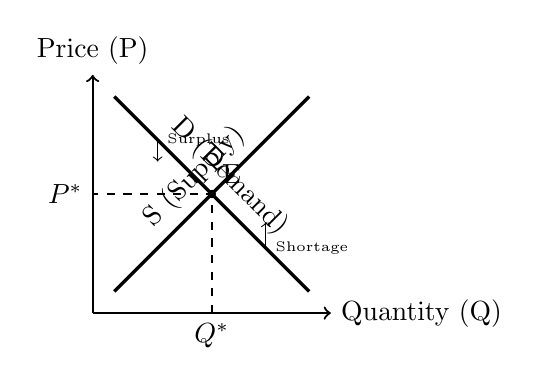
\begin{tikzpicture}[scale=0.55, thick]
    % Axes
    \draw[->] (0,0) -- (5.5,0) node[right] {Quantity (Q)};
    \draw[->] (0,0) -- (0,5.5) node[above] {Price (P)};
    % Demand curve
    \draw[very thick] (0.5,5) -- (5,0.5) node[midway, above, sloped] {D (Demand)};
    % Supply curve
    \draw[very thick] (0.5,0.5) -- (5,5) node[midway, above, sloped] {S (Supply)};
    % Equilibrium point
    \filldraw (2.75,2.75) circle (2pt) node[above right] {E};
    \draw[dashed] (2.75,0) node[below] {$Q^*$} -- (2.75,2.75) -- (0,2.75) node[left] {$P^*$};
    % Surplus region
    \draw[->, thin] (1.5,4) node[right] {\tiny Surplus} -- (1.5,3.5);
    % Shortage region
    \draw[->, thin] (4,1.5) node[right] {\tiny Shortage} -- (4,2.1);
\end{tikzpicture}
\end{center}
\textit{Interpretation:} At $P > P^*$, surplus drives price down. At $P < P^*$, shortage drives price up. Market forces push toward equilibrium automatically.

% --- MOVEMENTS vs SHIFTS ---
\subsection*{Movements Along vs. Shifts}
\begin{center}
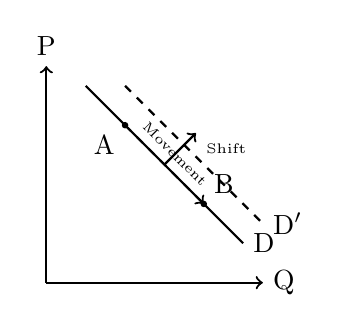
\begin{tikzpicture}[scale=0.5, thick]
    % Axes
    \draw[->] (0,0) -- (5.5,0) node[right] {Q};
    \draw[->] (0,0) -- (0,5.5) node[above] {P};
    % Demand curve
    \draw (1,5) -- (5,1) node[right] {D};
    % Movement along
    \filldraw (2,4) circle (1.5pt) node[below left] {A};
    \filldraw (4,2) circle (1.5pt) node[above right] {B};
    \draw[->, dashed] (2,4) -- (4,2) node[midway, above, sloped] {\tiny Movement};
    % Shift right
    \draw[dashed] (2,5) -- (5.5,1.5) node[right] {D$'$};
    \draw[->] (3,3) -- (3.8,3.8) node[below right] {\tiny Shift};
\end{tikzpicture}
\end{center}
\textbf{Movement:} Caused by change in own price (contraction/expansion).\\
\textbf{Shift:} Caused by non-price determinants (increase/decrease in demand/supply).

\columnbreak

% --- FACTORS INFLUENCING ---
\section*{Factors Influencing Demand \& Supply}

\subsection*{Demand Determinants (Shifters)}
\begin{enumerate}[leftmargin=*,nosep]
    \item \textbf{Income:} Normal goods (demand $\uparrow$ with income); Inferior goods (demand $\downarrow$).
    \item \textbf{Prices of Related Goods:} Substitutes (tea $\uparrow$ $\to$ coffee demand $\uparrow$); Complements (car $\uparrow$ $\to$ petrol demand $\downarrow$).
    \item \textbf{Tastes \& Preferences:} Trends, advertising, seasons.
    \item \textbf{Expectations:} Future price rise $\to$ current demand $\uparrow$.
    \item \textbf{Number of Buyers:} Population growth $\to$ demand $\uparrow$.
    \item \textbf{Government Policies:} Taxes, subsidies.
\end{enumerate}

\subsection*{Supply Determinants (Shifters)}
\begin{enumerate}[leftmargin=*,nosep]
    \item \textbf{Input/Cost of Production:} Raw material, labor cost $\uparrow$ $\to$ supply $\downarrow$.
    \item \textbf{Technology:} Improvement $\to$ supply $\uparrow$.
    \item \textbf{Prices of Related Goods in Production:} Substitutes in supply (wheat vs corn).
    \item \textbf{Expectations:} Future price $\uparrow$ $\to$ current supply $\downarrow$ (withhold).
    \item \textbf{Number of Sellers:} More firms $\to$ market supply $\uparrow$.
    \item \textbf{Natural Factors:} Weather, disasters (especially agriculture).
    \item \textbf{Government Policies:} Subsidies $\uparrow$ supply; taxes $\downarrow$ supply.
\end{enumerate}

% --- SCHEDULES ---
\subsection*{Demand \& Supply Schedules}
\textit{Individual Demand Schedule (Orange Market):}
\begin{center}
\begin{tabular}{|c|c|}
\hline
Price (\$/kg) & Qty Demanded (kg/week) \\
\hline
5 & 2 \\
4 & 4 \\
3 & 6 \\
2 & 8 \\
1 & 10 \\
\hline
\end{tabular}
\end{center}
\textit{Market Supply Schedule (Orange Market):}
\begin{center}
\begin{tabular}{|c|c|}
\hline
Price (\$/kg) & Qty Supplied (kg/week) \\
\hline
5 & 12 \\
4 & 10 \\
3 & 8 \\
2 & 6 \\
1 & 4 \\
\hline
\end{tabular}
\end{center}
\textbf{Market Demand/Supply:} Horizontal summation of all individual demand/supply curves at each price. $Q_{\text{market}} = \sum Q_{\text{individual}}$.

% --- LAW OF DEMAND ---
\subsection*{Law of Demand}
\textit{Ceteris paribus}, there is an \textbf{inverse relationship} between price and quantity demanded.
\begin{itemize}[leftmargin=*,nosep]
    \item \textbf{Reasons:} Income effect (purchasing power), Substitution effect (relatively cheaper alternatives).
    \item \textbf{Exceptions (Giffen/Veblen goods):} Price $\uparrow$ $\to$ demand $\uparrow$ (rare).
\end{itemize}

% --- EFFECTS OF SHIFTS ON EQUILIBRIUM ---
\subsection*{Shifts Effects on Equilibrium}
\begin{center}
\begin{tabular}{|c|c|c|c|}
\hline
\textbf{Change} & \textbf{D} & \textbf{S} & \textbf{P*, Q*} \\
\hline
D $\uparrow$ & Shift right & Constant & P $\uparrow$, Q $\uparrow$ \\
D $\downarrow$ & Shift left & Constant & P $\downarrow$, Q $\downarrow$ \\
S $\uparrow$ & Constant & Shift right & P $\downarrow$, Q $\uparrow$ \\
S $\downarrow$ & Constant & Shift left & P $\uparrow$, Q $\downarrow$ \\
\hline
\end{tabular}
\end{center}
\textbf{Simultaneous Shifts:} Effect on P and Q depends on relative magnitudes of shifts (draw graphs).

% --- SPECIAL CASES ---
\subsection*{Special Cases}
\begin{enumerate}[leftmargin=*,nosep]
    \item \textbf{Perfectly Inelastic Demand ($Q_d$ fixed):} Vertical demand curve (e.g., life-saving drug). Supply shift only changes price, quantity unchanged.
    \item \textbf{Perfectly Elastic Demand:} Horizontal demand curve (e.g., identical products in perfect competition). Any price above market $\to$ demand zero.
    \item \textbf{Price Floor (Minimum Price):} Set above equilibrium $\to$ persistent surplus (e.g., agricultural support price).
    \item \textbf{Price Ceiling (Maximum Price):} Set below equilibrium $\to$ persistent shortage (e.g., rent control).
    \item \textbf{Black Markets:} Emerge under binding price ceilings where goods sell at illegal higher prices.
\end{enumerate}

% --- CASE STUDIES ---
\subsection*{Case Studies}
\begin{enumerate}[leftmargin=*,nosep]
    \item \textbf{Housing Crisis \& Rent Control (New York, WWII):} Price ceiling on rents kept housing below market rate. Result: Persistent \textbf{shortage} of rental units, deterioration of buildings, black market sublets. \textit{Concept:} Binding price ceiling below equilibrium creates excess demand.
    \item \textbf{Global Semiconductor Shortage (2020--2022):} COVID disrupted supply chains ($S \downarrow$), while demand for electronics spiked with remote work ($D \uparrow$). Result: Prices rose sharply, auto industry stalled. \textit{Concept:} Simultaneous leftward supply shift and rightward demand shift $\to$ unambiguously higher price, ambiguous quantity effect (here Q fell due to dominant supply shock).
\end{enumerate}

% --- EXAM QUESTIONS ---
\subsection*{Exam Practice}
\textbf{Q1:} The demand and supply functions for a good are: $Q_d = 100 - 5P$ and $Q_s = 20 + 3P$. Find equilibrium price and quantity.\\[0.1cm]
\textbf{Answer:} Set $Q_d = Q_s$: $100 - 5P = 20 + 3P \Rightarrow 8P = 80 \Rightarrow \mathbf{P^* = 10}$. $Q^* = 100 - 5(10) = \mathbf{50}$ units.\\[0.2cm]

\textbf{Q2:} Distinguish between a ``movement along'' and a ``shift in'' the demand curve using an example.\\[0.1cm]
\textbf{Answer:} A movement along occurs when own price changes (e.g., price of apples falls from \$3 to \$2 $\to$ quantity demanded rises -- Law of Demand). A shift occurs when a non-price determinant changes (e.g., health study reveals apples reduce disease risk $\to$ demand curve shifts right, more bought at every price).\\[0.2cm]

\textbf{Q3:} Explain the effect of a government subsidy to wheat farmers on the equilibrium price and quantity of wheat. Illustrate.\\[0.1cm]
\textbf{Answer:} A subsidy reduces production costs, shifting the \textbf{supply curve rightward} ($S \to S'$). This creates surplus at original price, driving price \textbf{down} and equilibrium quantity \textbf{up}. Consumers benefit from lower prices; producers receive price + subsidy.
\end{multicols}
\end{document}